\documentclass[12pt]{article}
\usepackage[utf8]{inputenc}
\usepackage{amsmath}
\usepackage{soul}
\usepackage{xcolor}
\usepackage{amssymb}
\usepackage{float}
\usepackage{graphicx}
\usepackage{geometry}
\usepackage{framed} % For the box
\sethlcolor{yellow}
\newcommand{\red}[1]{\textcolor{red}{#1}}
\newcommand{\blue}[1]{\textcolor{blue}{#1}}

% Adjust margins
\geometry{margin=1in}

\title{\textbf{CSE421: Design and Analysis of Algorithms}}
\author{Homework 1 \\ Shaqan Oveis Gharan}
\date{March 27th, 2024 \\ Due: April 3rd, 2024 at 11:59 PM}


\begin{document}

\noindent CS-3510-\textbf{\red{Your Section\#}} Algorithms, Spring 2025\hfill Mid-Term 1 Take-Home\\
\blue{FirstName} \blue{LastName} \hfill Collaborator(s):

\hrulefill

\subsection*{Problem 1 (10 pts)}
For this problem, we explore the issue of \textit{truthfulness} in the Gale-Shapley algorithm for Stable Matching. Show that a participant can improve its outcome by lying about its preferences. Consider $r \in R$. Suppose $r$ prefers $p$ to $p'$, but $p$ and $p'$ are low on $r$'s preference list. Show that it is possible that by switching the order of $p$ and $p'$ on $r$'s preference list, $r$ achieves a better outcome, e.g., is matched with a $p''$ higher on the preference list than the one if the actual order was used.

\textit{Hint:} Prove the claim by finding one specific instance of stable matching problem and comparing the stable matching before and after the switching.

\subsection*{Problem 2 (10 pts)}
Arrange in increasing order of asymptotic growth. All logs are in base 2.

\begin{enumerate}
    \item \( n^{\frac{5}{3}} \log^2 n \)
    \item \( 2^{\sqrt{\log n}} \)
    \item \( \sqrt{n^n} \)
    \item \( \frac{n^2}{\log n} \)
    \item \( 2^n \)
\end{enumerate}


\subsection*{Problem 3 (10 pts)}
We say that $T(n)$ is $O(f(n))$ if there exist $c$ and $n_0$ such that for all $n > n_0,\:T(n) \le cf(n)$. Use this definition for parts $a$ and $b$.
\begin{enumerate}
    \item Prove that $4n^2 + 3n\text{log}\:n + 6n + 20\text{log}^2n + 11$ is $O(n^2)$. (You may use, without proof, the fact that $\text{log}\:n < n$ for $n \ge 1$.)
    \item Suppose that $f(n)$ is $O(r(n))$ and $g(n)$ is $O(s(n))$. Let $h(n) = f(n)g(n)$ and $t(n) = r(n)s(n)$. Prove that $h(n)$ is $O(t(n))$.
\end{enumerate}

\subsection*{Problem 4 (10 pts)}
The \textit{diameter} of an undirected graph is the maximum distance between any pair of vertices. If a graph is not connected, its diameter is infinite. Let $G$ be an $n$ node undirected graph, where $n$ is even. Suppose that every vertex has degree at least n/2. Prove that G has diameter at most 2.

\textit{Hint:} Proof by contradiction

\subsection*{Problem 5 (10 pts)}
Show that there are at least $3\cdot2^{n-1}$ ways to properly color vertices of a tree T with n vertices using 3 colors, i.e., to color vertices with three colors such that any two adjacent vertices have  distinct colors. Note that it can be shown that there are exactly $3\cdot2^{n-1}$ ways to properly color vertices of T with 3 colors but in this problem, to receive full credit, it is enough prove the “at least” part.\\
For example, there are (at least) $3\cdot2^2 = 12$ ways to color a tree with 3 vertices as show below:

\begin{figure}[H]
    \centering
    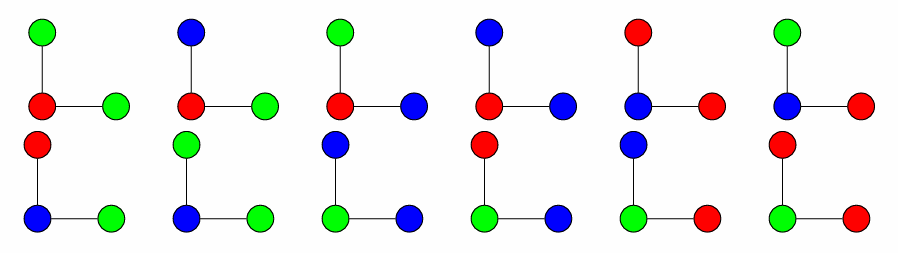
\includegraphics[width=0.8\linewidth]{P5.png}
    \label{fig:3-color-graph}
\end{figure}

\subsection*{Problem 6 (Extra Credit: 10 pts)}
Given a directed graph $G$ with $n$ vertices $V = \{1,2,\cdots,n\}$ and $m$ edges. We say that a vertex $j$ is reachable from $i$ if there is a directed path from $i$ to $j$. Design an $O(m+n)$-time algorithm (show the pseudo-code) that for any vertex $i$ outputs the smallest label reachable from $i$. For example, given the following graph you should output 1,2,2,2,1 corresponding to the smallest indices reachable from vertices 1,2,3,4,5 respectively.
\begin{figure}[H]
    \centering
    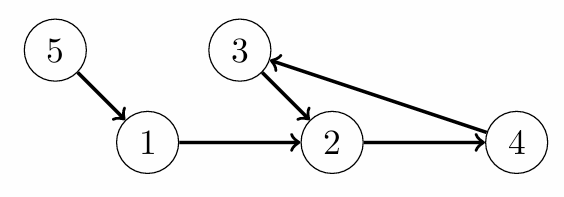
\includegraphics[width=0.5\linewidth]{P6.png}
    \label{fig:P6}
\end{figure}

\end{document}


